\documentclass[dvipsnames]{beamer} % Use handout option to remove pauses.
\usetheme{default}
\usefonttheme{structurebold}
\usefonttheme[onlymath]{serif}
\usepackage[UKenglish,cleanlook]{isodate}                                  % Set default date and date display
\usepackage[T1]{fontenc}
% Slide title background color
\definecolor{background}{HTML}{ede6d8}
% Slide title text color
\definecolor{titleText}{HTML}{B40404}
% Add slide numbers in bottom right corner
\defbeamertemplate{headline}{my header}{
    \vskip1pt
    \makebox[0pt][l]{\,\insertsection}
    \hspace*{\fill}\insertshorttitle\hspace*{\fill}
    \llap{\insertframenumber\,/\,\inserttotalframenumber\,}
}
\setbeamertemplate{headline}[my header]
% Add name at the bottom
\setbeamercolor{footlinecolor}{fg=black,bg=background}
\defbeamertemplate{footline}{my footer}{%
    \begin{beamercolorbox}[wd=\paperwidth,leftskip=0.25cm,rightskip=0.25cm]{footlinecolor}
        \insertshortauthor
        \hfill
        \insertframenumber{} / \inserttotalframenumber
    \end{beamercolorbox}
}
\setbeamertemplate{footline}[my footer]
\setbeamertemplate{navigation symbols}[default]
\usepackage{graphicx}
% Set font sizes for frame title and subtitle
\setbeamerfont{frametitle}{size=\fontsize{15}{16}}
\setbeamerfont{framesubtitle}{size=\small}
% Set left and right text margins
\setbeamersize{text margin left=5mm, text margin right=5mm}
\usepackage{booktabs,multirow}
\usepackage{subcaption}   % Sub figures.
\usepackage{tikz}
\usetikzlibrary{shapes,decorations,decorations.pathreplacing,arrows,calc,arrows.meta,fit,positioning}
\tikzset{
    auto,node distance =1 cm and 1 cm,semithick,
    state/.style ={ellipse, draw, minimum width = 0.7 cm},
    point/.style = {circle, draw, inner sep=0.04cm,fill,node contents={}},
    bidirected/.style={Latex-Latex,dashed},
    el/.style = {inner sep=2pt, align=left, sloped}
}
\usepackage{mathtools}                                                     % Various maths functions
\usepackage{amssymb}                                                       % Various maths functions
\usepackage{amsmath}                                                       % Various maths functions
\usepackage{dsfont}                                                        % Various maths functions
\usepackage{centernot}                                                     % center \not usage
\usepackage{siunitx} \sisetup{round-mode=places, round-precision=3}        % Formalise use of units and numbers among text
\usepackage[normalem]{ulem} % Strike-through package
\renewcommand{\vec}[1]{\boldsymbol{\mathit{#1}}}                           % vector notation shortcut
\newcommand{\mat}[1]{\boldsymbol{\mathit{#1}}}                             % matrix notation shortcut
\DeclarePairedDelimiter\abs{\lvert}{\rvert}                                % absolute value notation shortcut
\DeclarePairedDelimiter\norm{\lVert}{\rVert}                               % norm notation shortcut
\newcommand{\Prob}[1]{\Pr\left( #1 \right)}                         % SHortcut for probability notation
\newcommand{\Probgiven}[2]{\Pr\left( #1 \, \middle\vert \, #2 \right)} % SHortcut for probability notation, given
\newcommand{\E}[2][]{\mathbb{E}_{#1} \left[ #2 \right]}                    % Expectation (with optional subscript) shortcut
\newcommand{\Egiven}[3][]{\mathbb{E}_{#1} \left[ #2 \, \middle\vert \, #3 \right]} % Expectation given (with optional subscript) shortcut
\newcommand{\Var}[2][]{\text{Var}_{#1} \left( #2 \right)}                  % Variation (with optional subscript) shortcut
\newcommand{\Cov}[1]{\text{Cov} \left( #1 \right)}                         % Covariance (with optional subscript) shortcut
\newcommand{\indicator}[1]{\mathds{1}\left\{ #1 \right\}}                  % SHortcut for indicator function
\newcommand{\indep}{\, \raisebox{0.05em}{\rotatebox[origin=c]{90}{$\models$}} \,}% Statistical independence symbol.
\newcommand{\diff}[2][]{\frac{d#1}{d#2}}                                   % SHortcut for differential fraction as a function
\newcommand{\partialdiff}[2][]{\frac{\partial#1}{\partial#2}}              % SHortcut for partial differential fraction as a function
\renewcommand{\hat}[1]{\widehat{#1}}                                       % Default estimator notation is widehat
\renewcommand{\bar}[1]{\overline{#1}}                                      % Make over bar look nicer
\renewcommand{\tilde}[1]{\widetilde{#1}}                                   % Make over tilde look better
% Citations
\usepackage{natbib}                                        % Citation package, see https://en.wikibooks.org/wiki/LaTeX/Bibliography_Management#Natbib
\usepackage{hyperref}                                        % Allow for links across the text, with colour options
\usepackage{setspace}
\settowidth{\leftmargini}{\usebeamertemplate{itemize item}}
\addtolength{\leftmargini}{\labelsep}
\usepackage{soul,color,xcolor} % Text highlighting
\newcommand{\eqhighlight}[2]{\colorbox{#1!50}{$\displaystyle#2$}}
\makeatletter
\let\HL\hl
\renewcommand\hl{%
    \let\set@color\beamerorig@set@color
    \let\reset@color\beamerorig@reset@color
    \HL}
\makeatother
\newcommand{\mathcolorbox}[2]{\colorbox{#1}{$\displaystyle #2$}}
% Set colors
\setbeamercolor{block title}{use=structure,fg=white,bg=structure.fg!75!black}
\setbeamercolor{block body}{parent=normal text,use=block title,bg=block title.bg!10!bg}
\setbeamercovered{transparent}
\setbeamercolor{postit}{fg=black, bg=yellow}
\setbeamercolor{frametitle}{bg=background, fg=titleText}
\setbeamercolor{subtitle}{fg=titleText}
% Command to align text
\renewcommand{\raggedright}{\leftskip=0pt \rightskip=0pt plus 0cm}
% Remove the useless buttons.
\setbeamertemplate{navigation symbols}{}
\useoutertheme[footline=empty,subsection=false]{miniframes}
\useinnertheme{circles}
% Line up a QR code to the document.
\usepackage{qrcode}
% \qrcode[height=1.5cm]{https://https://shoganhennessy.github.io/}

%-------------------------------------------------------------------------------
% Title Page
%-------------------------------------------------------------------------------
\title{\color{titleText}
    \href{https://raw.githubusercontent.com/shoganhennessy/mediation-natural-experiment/main/mediation-natural-experiment-2025.pdf}{Causal Mediation in Natural Experiments}
}
\author[Senan Hogan-Hennessy, Cornell University]{
    Senan Hogan-Hennessy \\
    Economics Department, Cornell University   \\ %\vspace{0.5cm}
    \href{mailto:seh325@cornell.edu}{\textcolor{blue}{seh325@cornell.edu}}
}
\date{} % Date, can be changed to a custom date

%-------------------------------------------------------------------------------
% Opening Slides
\begin{document}
% Justify text through-out.
\raggedright
%-------------------------------------------------------------------------------
%% Title page
\begin{frame}[noframenumbering, plain]
    % Print the title page as the first slide
    \vspace{1.5cm}
    \titlepage
    \begin{center}
        \vspace{-1.5cm}
        
\includegraphics[width=2cm]{presentation-files/cornell}

        %\vspace{0.5cm}
        \vskip0pt plus 1filll
        \par\noindent\rule{\textwidth}{0.4pt}
        Cornell Economics, PhD Defence \\
        29 June 2026
    \end{center}
\end{frame}
%-------------------------------------------------------------------------------
\begin{frame}
    \frametitle{Introduction}
    \textbf{Motivation:}
    \begin{itemize}
        \item Causal Mediation (CM) is a framework for studying mechanisms of causal effects, but is not widely used in economics 
        \item Economists stick to \textit{suggestive evidence}, leaving mechanisms not identified.
    \end{itemize}
    
    \pause
    \textbf{Contribution:}
    \begin{itemize}
        \item Develop selection bias concept for CM, crystallising reasoning for economists' dismissal of these methods
        \item Develop a Marginal Treatment Effect (MTE) approach to credibly estimate causal channels (direct and indirect effects).
    \end{itemize}

    \pause
    \par\noindent\rule{\textwidth}{0.4pt}
    \textbf{Key findings:}
    \begin{itemize}
        \item Apply methods to the Oregon Health Insurance Experiment, studying mediating role of healthcare take-up
        \item Bring CM into economic quasi-experimental causal inference.
    \end{itemize}
\end{frame}
%-------------------------------------------------------------------------------
\section{1. Suggestive Evidence}
\begin{frame}
    \frametitle{1. Suggestive Evidence}
    In 2008, Oregon gave access to socialised health insurance by wait-list lottery (Finkelstein et al, 2012).
    \begin{figure}
        \caption{Model for Suggestive Evidence of a Mechanism.}
        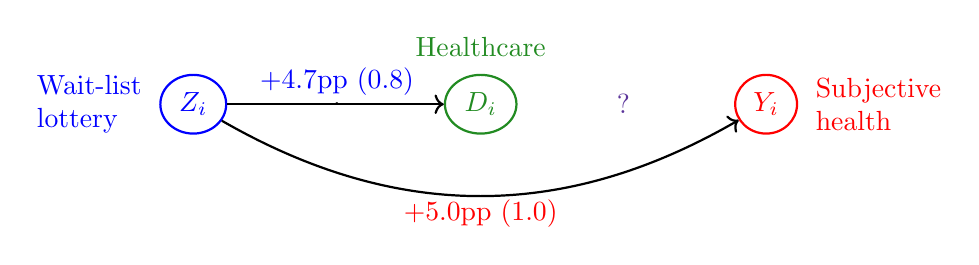
\begin{tikzpicture}
            \node[state,thick,ForestGreen] (mediator) at (0,0) {$D_i$};
            \node[state,thick,blue] (treatment) [left=2.75cm of mediator] {$Z_i$};
            \node[state,thick,red] (outcome)   [right=2.75cm of mediator] {$Y_i$};
            % Label Z_i, D, Y_i
            \node[color=ForestGreen] [above=0.1cm of mediator] {Healthcare};
            \node[color=blue,align=left] [left=0.1cm of treatment] {Wait-list \\ lottery};
            % Draw the causal arrows
            \path[->, thick] (treatment) edge (mediator);
            %\path[->, dashed,color=gray] (mediator) edge (outcome);
            \node[color=black] (firststage) at ($(mediator)!0.5!(treatment)$) {.};
            \node[color=blue] [above=-0.15cm of firststage] {+4.7pp (0.8)};
            \pause
            \node[color=red,align=left] [right=0.1cm of outcome] {Subjective \\ health};
            \path[->, thick] (treatment) edge[bend right=30] (outcome);
            \node[color=red] [below=0.7cm of mediator] {+5.0pp (1.0)};
            % Label the problem.
            \node[color=RoyalPurple] at ($(mediator)!0.5!(outcome)$) {?};
        \end{tikzpicture}
    \end{figure}
    
    \vfill
    \pause
    \par\noindent\rule{\textwidth}{0.4pt}
    \textbf{Necessary but not sufficient evidence on the mediating mechanism:}
    \vskip-0.01cm
    \begin{itemize}
        \item Is $\textcolor{ForestGreen}{D_i} \to \textcolor{red}{Y_i}$ small, large, non-zero?
        \item Can we assume a causal effect (among healthcare-lottery switchers)?
    \end{itemize}
\end{frame}
%-------------------------------------------------------------------------------
\section{2. Causal Mediation}
\begin{frame}
    \frametitle{2. Causal Mediation}
    Causal Mediation (CM) models the entire system, giving sufficient evidence on the mediating mechanism.
    \vskip-0.5cm
    \begin{figure}
        \centering
        \singlespacing
        
\begin{tikzpicture}
            \node (mediator) at (0,0) {};
            \node[state, thick,blue] (treatment) [left=2cm of mediator] {$Z_i$};
            \node[state, thick,red] (outcome) [right=2cm of mediator] {$Y_i$};
            % Label Z, D, Y
            \node[color=blue] [left=0.1cm of treatment] {Wait-list lottery};
            \node[color=red,align=left] [right=-0.01cm of outcome]  {Subjective \\ health};
            % Draw the causal arrows
            \path[->, thick] (treatment) edge (outcome);
            % Label direct and indirect effect
            \node[color=orange] [above=-0.125cm of mediator] {Treatment Effect (ATE)};
        \end{tikzpicture}
    \end{figure}
    
    \vskip0.75cm
    \par\noindent\rule{\textwidth}{0.4pt}
    \textcolor{gray!25}{
    Average Direct Effect (ADE) and Average Indirect Effect (AIE):}
    %\[ \text{Average Direct Effect (ADE)}: \;\;\;
    %    \E{Y_i\left(\eqhighlight{blue}{1}, D_i(Z_i) \right)
    %        - Y_i\left(\eqhighlight{blue}{0}, D_i(Z_i) \right)} \]
    %\vskip-0.35cm
    \begin{itemize}
        \item \textcolor{gray!25}{ADE is causal effect $Z_i \to Y_i$}
        \item \textcolor{gray!25}{AIE is causal effect of $D_i(Z_i) \to Y_i$.}
    \end{itemize}
    %\[ \text{Average Indirect Effect (AIE):} \;\;\;
    %\E{Y_i\left(Z_i, \eqhighlight{ForestGreen}{D_i(1)} \right)
    %    - Y_i\left(Z_i, \eqhighlight{ForestGreen}{D_i(0)} \right)} \]
    \pause
    \par\noindent\rule{\textwidth}{0.4pt}
    \textcolor{gray!25}{
    \textbf{Identification:} Requires mediator $D_i$ is quasi-randomly assigned$\hdots$.}
\end{frame}
%-------------------------------------------------------------------------------
\begin{frame}[noframenumbering]
    \frametitle{2. Causal Mediation}
    Causal Mediation (CM) models the entire system, giving sufficient evidence on the mediating mechanism.
    \vskip-0.5cm
    \begin{figure}
        \centering
        \singlespacing
        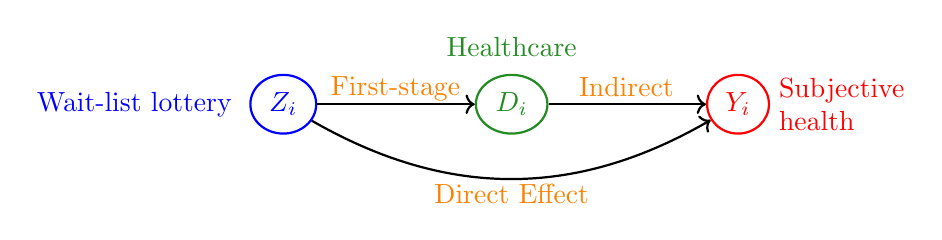
\begin{tikzpicture}
            \node[state, thick,ForestGreen] (mediator) at (0,0) {$D_i$};
            \node[state, thick,blue] (treatment) [left=2cm of mediator] {$Z_i$};
            \node[state, thick,red] (outcome) [right=2cm of mediator] {$Y_i$};
            % Label Z, D, Y
            \node[color=ForestGreen] [above=0.1cm of mediator] {Healthcare};
            \node[color=blue] [left=0.1cm of treatment] {Wait-list lottery};
            \node[color=red,align=left] [right=-0.01cm of outcome]  {Subjective \\ health};
            % Draw the causal arrows
            \path[->, thick] (treatment) edge (mediator);
            \path[->, thick] (mediator) edge (outcome);
            \path[->, thick] (treatment) edge[bend right=30] (outcome);
            % Label direct and indirect effect
            \node[color=orange] [above left=-0.35cm and 0.2cm of mediator] {First-stage};
            \node[color=orange] [above right=-0.3cm and 0.4cm of mediator] {Indirect};
            \node[color=orange] [below=0.5cm of mediator] {Direct Effect};
        \end{tikzpicture}
    \end{figure}
    \vskip-0.5cm
    \pause
    \par\noindent\rule{\textwidth}{0.4pt}
    Average Direct Effect (ADE) and Average Indirect Effect (AIE):
    %\[ \text{Average Direct Effect (ADE)}: \;\;\;
    %    \E{Y_i\left(\eqhighlight{blue}{1}, D_i(Z_i) \right)
    %        - Y_i\left(\eqhighlight{blue}{0}, D_i(Z_i) \right)} \]
    %\vskip-0.35cm
    \begin{itemize}
        \item ADE is causal effect $\textcolor{blue}{Z_i} \to \textcolor{red}{Y_i}$
        \item AIE is causal effect of $\textcolor{ForestGreen}{D_i(Z_i)} \to \textcolor{red}{Y_i}$.
    \end{itemize}
    %\[ \text{Average Indirect Effect (AIE):} \;\;\;
    %\E{Y_i\left(Z_i, \eqhighlight{ForestGreen}{D_i(1)} \right)
    %    - Y_i\left(Z_i, \eqhighlight{ForestGreen}{D_i(0)} \right)} \]
    \par\noindent\rule{\textwidth}{0.4pt}
    \textbf{Identification:} Requires \textcolor{ForestGreen}{mediator $D_i$} is quasi-randomly assigned$\hdots$.
\end{frame}
%-------------------------------------------------------------------------------
\begin{frame}
    \frametitle{2. Causal Mediation --- Selection Bias}
    \label{main:selection-bias}
    People chose to visit \textcolor{ForestGreen}{healthcare $D_i$} freely, not randomly assigned...
    \begin{figure}
        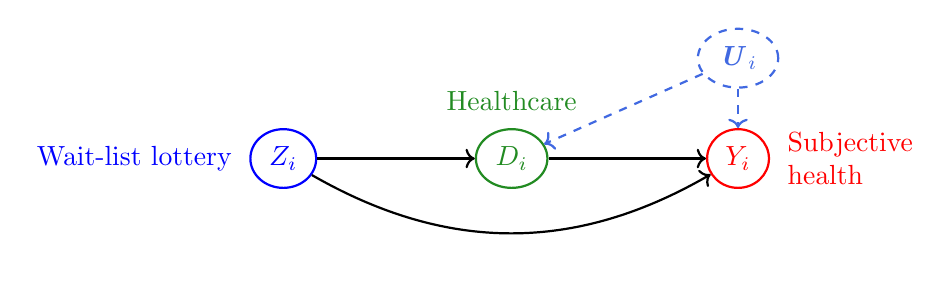
\begin{tikzpicture}
            \node[state,thick,ForestGreen] (mediator) at (0,0) {$D_i$};
            \node[state,thick,blue] (treatment) [left=2cm of mediator] {$Z_i$};
            \node[state,thick,red] (outcome)   [right=2cm of mediator] {$Y_i$};
            % Label Z_i, D, Y_i
            \node[color=ForestGreen] [above=0.1cm of mediator] {Healthcare};
            \node[color=blue] [left=0.1cm of treatment] {Wait-list lottery};
            \node[color=red,align=left] [right=0.1cm of outcome] {Subjective \\ health};
            % Draw the causal arrows
            \path[->, thick] (treatment) edge (mediator);
            \path[->, thick] (mediator) edge (outcome);
            \path[->, thick] (treatment) edge[bend right=30] (outcome);
            \pause
            \node[state, thick,dashed,thick,RoyalBlue] (confounderU) [
                above=0.5cm of outcome] {$\vec U_i$};
            \path[->,thick,dashed,color=RoyalBlue] (confounderU) edge (mediator);
            \path[->,thick,dashed,color=RoyalBlue] (confounderU) edge (outcome);
        \end{tikzpicture}
    \end{figure}
    \vskip-0.5cm
    \par\noindent\rule{\textwidth}{0.4pt}
    Conventional CM analyses are misleading in natural experiment settings --- I derive non-parametric selection bias terms for CM.
    %\hyperlink{cm-model}{\beamergotobutton{Model}}
    \begin{itemize}
        \item ADE:
        $ \;\;\ \text{\textcolor{purple}{CM Estimand}}
        = \text{\textcolor{blue}{ADE}}
            + \Big(\text{\textcolor{red}{Selection Bias}}
            + \text{\textcolor{orange}{Group difference bias}}\Big) $
        \item AIE:
        $ \;\;\;\; \text{\textcolor{purple}{CM Estimand}}
            = \text{\textcolor{ForestGreen}{AIE}}
            + \Big(\text{\textcolor{red}{Selection Bias}}
            + \text{\textcolor{orange}{Group difference bias}}\Big) $
        \hyperlink{group-diff-ade}{\beamergotobutton{ADE biases}}
        \hfill
        \hyperlink{group-diff-aie}{\beamergotobutton{AIE biases}}
    \end{itemize}
\end{frame}
%-------------------------------------------------------------------------------
\begin{frame}
    \frametitle{2. Causal Mediation --- Selection Bias}
    Simulations with cost-benefit selection-into-$\textcolor{ForestGreen}{D_i}$, CM estimates are biased.

    \makebox[\textwidth]{\parbox{1.25\textwidth}{
        \begin{figure}
            \vskip-0.25cm
            %\caption{Simulated Distribution of CM Effect Estimates from 10,000 DGPs.}
            %\vskip-0.25cm
            \begin{subfigure}[c]{0.525\textwidth}
                \centering
                \caption{$\hat{\text{ADE}} - \text{ADE}$.}
                \vskip-0.25cm
                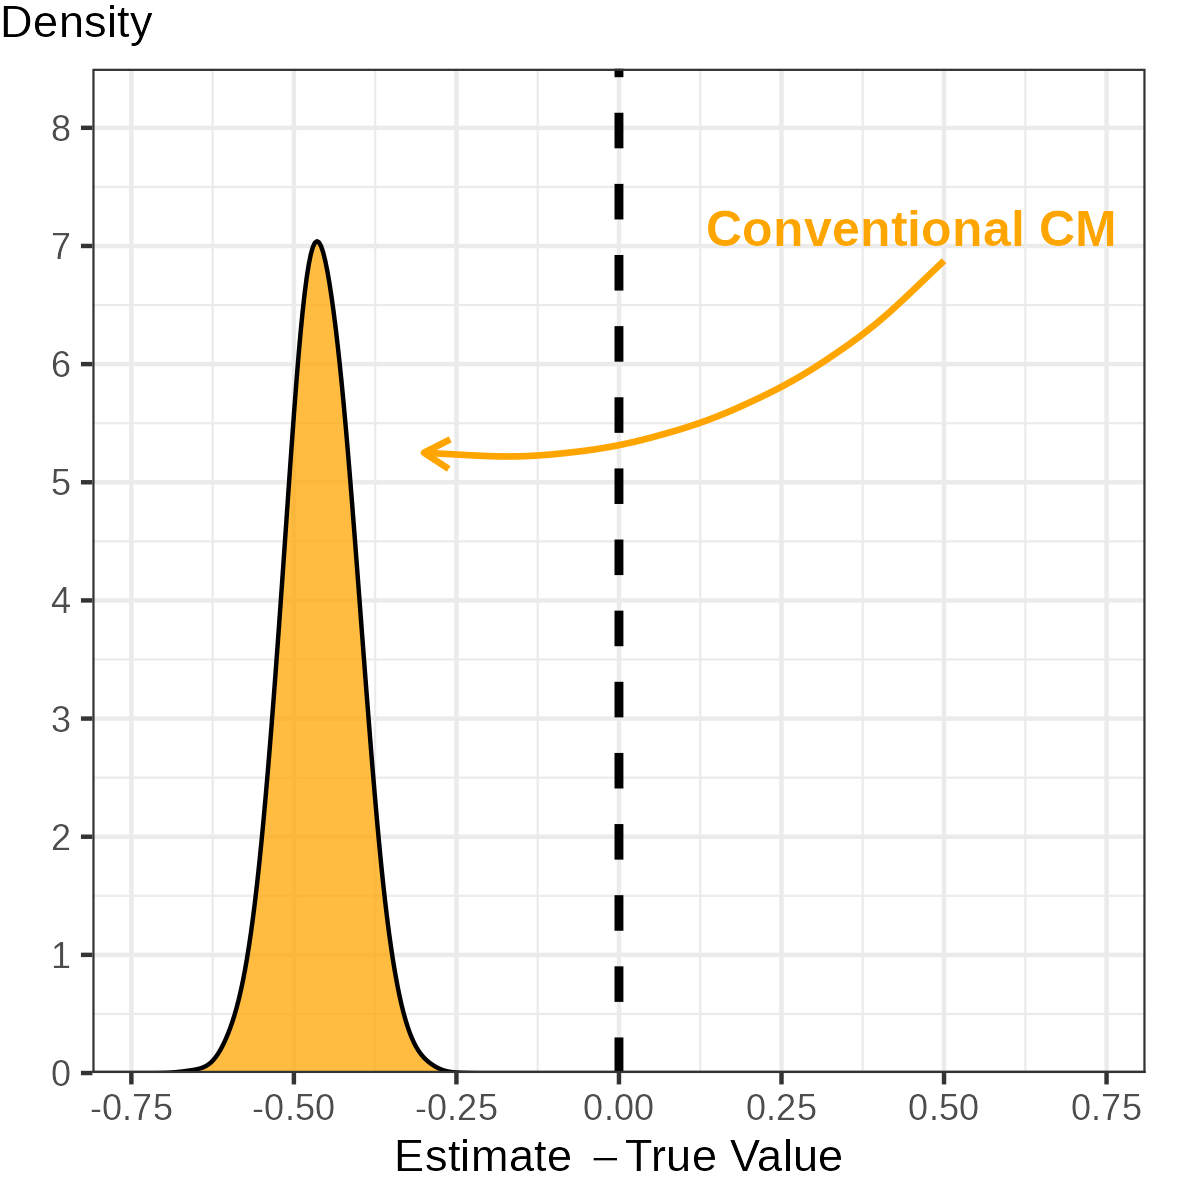
\includegraphics[width=\textwidth]{
                    ../text/sections/figures/ols-direct-dist.png}
            \end{subfigure}
            \begin{subfigure}[c]{0.525\textwidth}
                \centering
                \caption{$\hat{\text{AIE}} - \text{AIE}$.}
                \vskip-0.25cm
                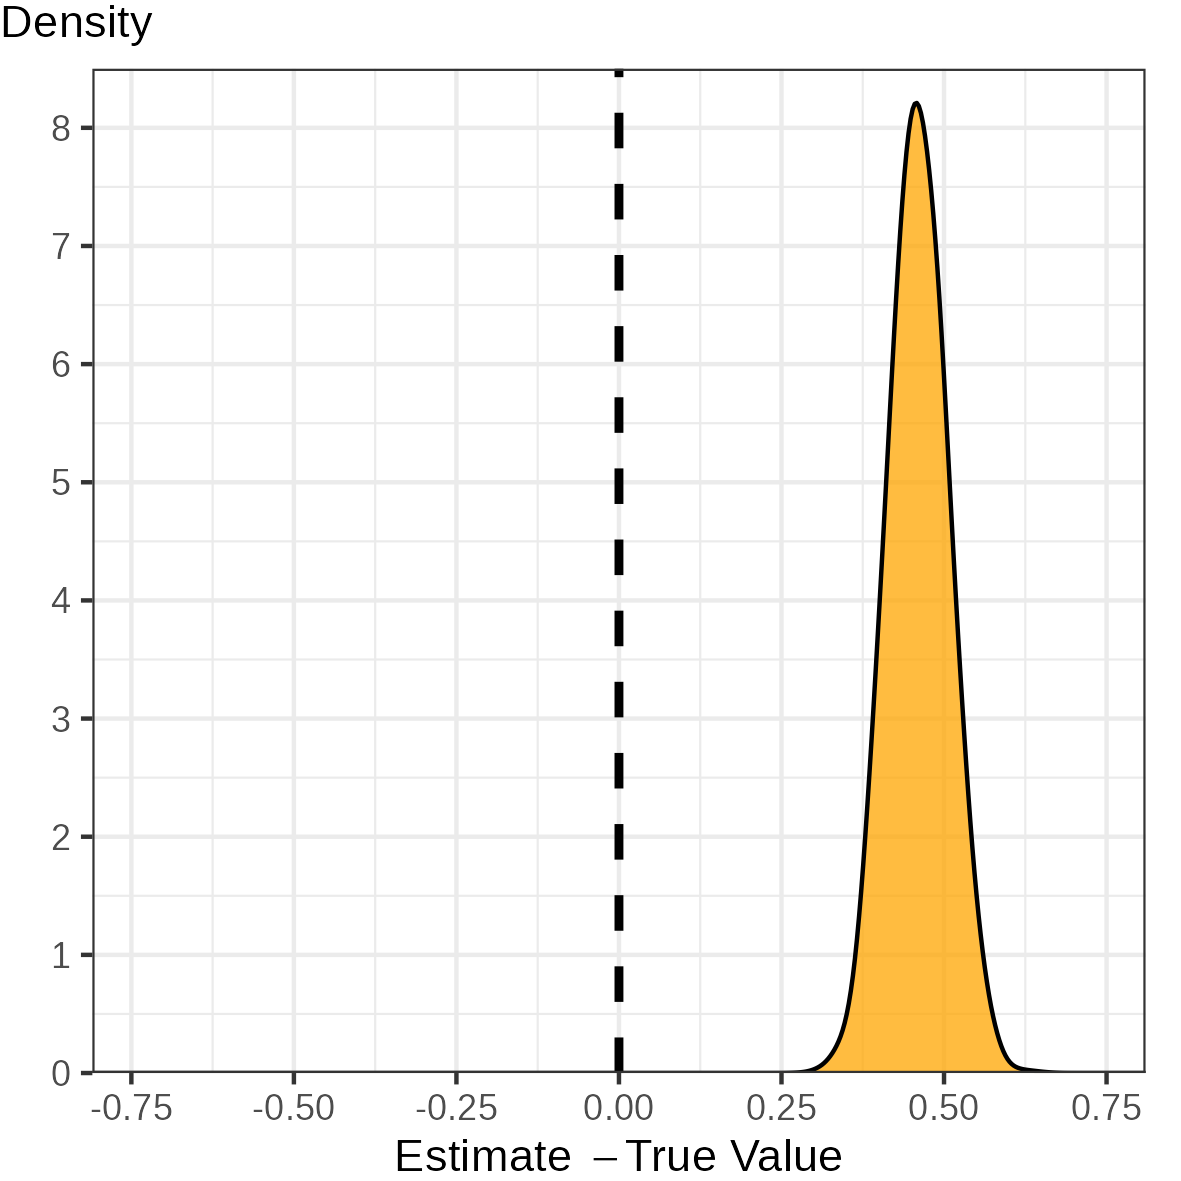
\includegraphics[width=\textwidth]{
                    ../text/sections/figures/ols-indirect-dist.png}
            \end{subfigure}
        \end{figure}
    }}
\end{frame}
%-------------------------------------------------------------------------------
\section{3. MTE Model}
\begin{frame}
    \frametitle{3. MTE Model}
    Conventional CM methods do not identify ADE $+$ AIE in a natural experiment setting, so I build a Marginal Treatment Effect (MTE) model. 

    \par\noindent\rule{\textwidth}{0.4pt}
    MTE model:

    \vskip-1.25cm
    \begin{figure}
        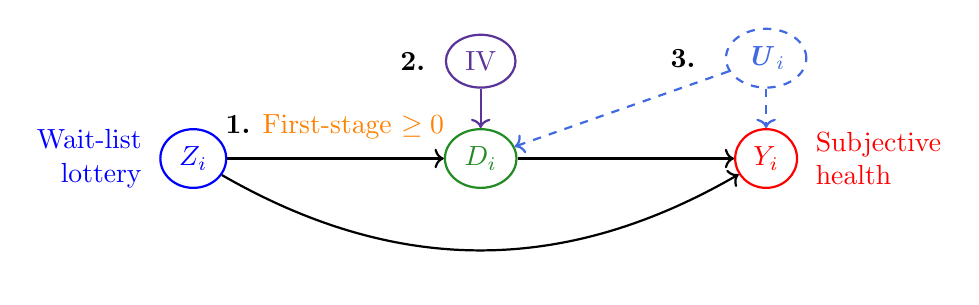
\begin{tikzpicture}
            \node[state,thick,ForestGreen] (mediator) at (0,0) {$D_i$};
            \node[state,thick,blue] (treatment) [left=2.75cm of mediator] {$Z_i$};
            \node[state,thick,red] (outcome)   [right=2.75cm of mediator] {$Y_i$};
            % Label Z_i, D, Y_i
            %\node[color=ForestGreen] [above=0.1cm of mediator] {Healthcare};
            \node[color=blue,align=right] [left=0.1cm of treatment] {Wait-list \\lottery};
            \node[color=red,align=left] [right=0.1cm of outcome] {Subjective \\ health};
            % Draw the causal arrows
            \path[->, thick] (treatment) edge (mediator);
            \path[->, thick] (mediator) edge (outcome);
            \path[->, thick] (treatment) edge[bend right=30] (outcome);
            \node[state, thick,dashed,thick,RoyalBlue] (confounderU) [
                above=0.5cm of outcome] {$\vec U_i$};
            % Label direct and indirect effects
            %\node[color=orange] [above right=-0.3cm and 0.75cm of mediator] {Indirect};
            %\node[color=orange] [below=0.75cm of mediator] {Direct Effect};
            \node[align=left] [above left=-0.15cm and 0.01cm of mediator] {\textbf{1.} \textcolor{orange}{First-stage $\geq 0$}};
            \node [left=0.25cm of confounderU] {\textbf{3.}};
            %\path[->,thick,dashed,color=white] (confounderU) edge (mediator);
            %\path[->,thick,dashed,color=RoyalBlue] (confounderU) edge (mediator);
            \path[->,thick,dashed,color=RoyalBlue] (confounderU) edge (mediator);
            \path[->,thick,dashed,color=RoyalBlue] (confounderU) edge (outcome);
            \node[state,thick,RoyalPurple] (instrument) [above=0.5cm of mediator] {IV};
            \path[->,thick,color=RoyalPurple] (instrument) edge (mediator);
            \node [left=0.125cm of instrument] {\textbf{2.}};
        \end{tikzpicture}
    \end{figure}
    
    \vskip-0.5cm

    \par\noindent\rule{\textwidth}{0.4pt}
    \begin{columns}[T]
        \begin{column}{0.3\textwidth}
            \textbf{MTE assumptions}:
        \end{column}
        % Column 2    
        \begin{column}{0.6\textwidth}
            \vskip-0.25cm
            \begin{enumerate}
                \item Mediator monotonicity
                \item IV for mediator take-up cost
                \item Selection on mediator benefits.
            \end{enumerate}
        \end{column}
    \end{columns}
    \vskip0.25cm
    \textbf{Intuition}:
    model $\textcolor{RoyalBlue}{\vec U_i}$ via mediator MTE to identify ADE $+$ AIE.
\end{frame}
%-------------------------------------------------------------------------------
\begin{frame}
    \frametitle{3. MTE Model}
    Simulation with cost-benefit selection-into-$\textcolor{ForestGreen}{D_i}$, MTE-model corrects for selection bias.
    \vskip-0.25cm
    \makebox[\textwidth]{\parbox{1.25\textwidth}{
        \begin{figure}
            %\caption{CM Estimates from 10,000 DGPs with \textbf{Normal} Errors.}
            \vskip-0.25cm
            \begin{subfigure}[c]{0.525\textwidth}
                \centering
                \caption{$\hat{\text{ADE}} - \text{ADE}$.}
                \vskip-0.25cm
                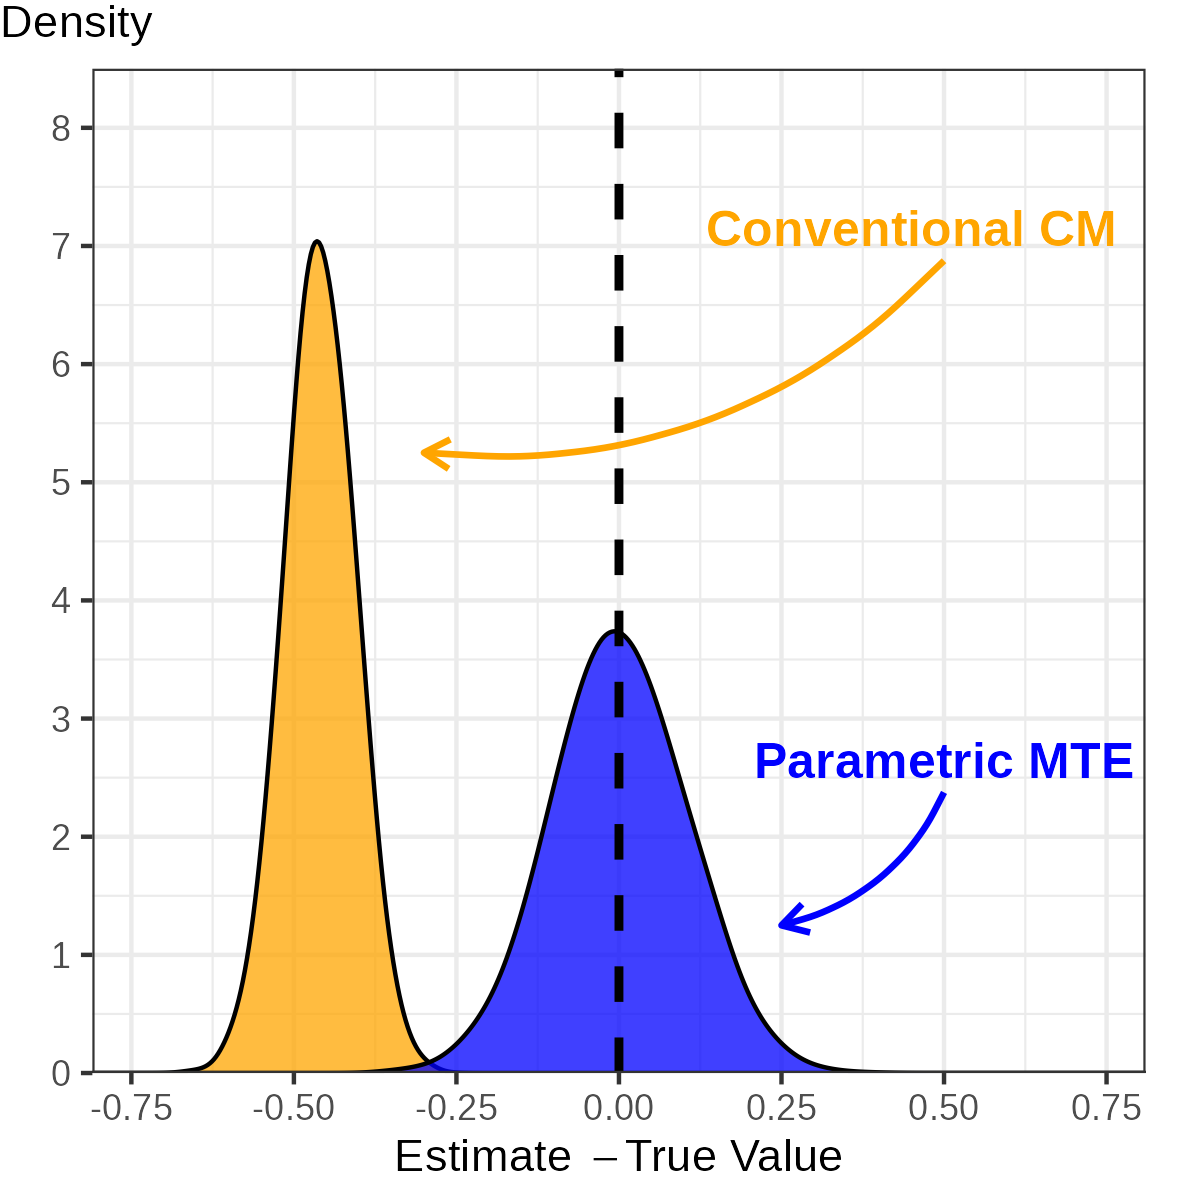
\includegraphics[width=\textwidth]{
                    ../text/sections/figures/normal-direct-dist.png}
            \end{subfigure}
            \begin{subfigure}[c]{0.525\textwidth}
                \centering
                \caption{$\hat{\text{AIE}} - \text{AIE}$.}
                \vskip-0.25cm
                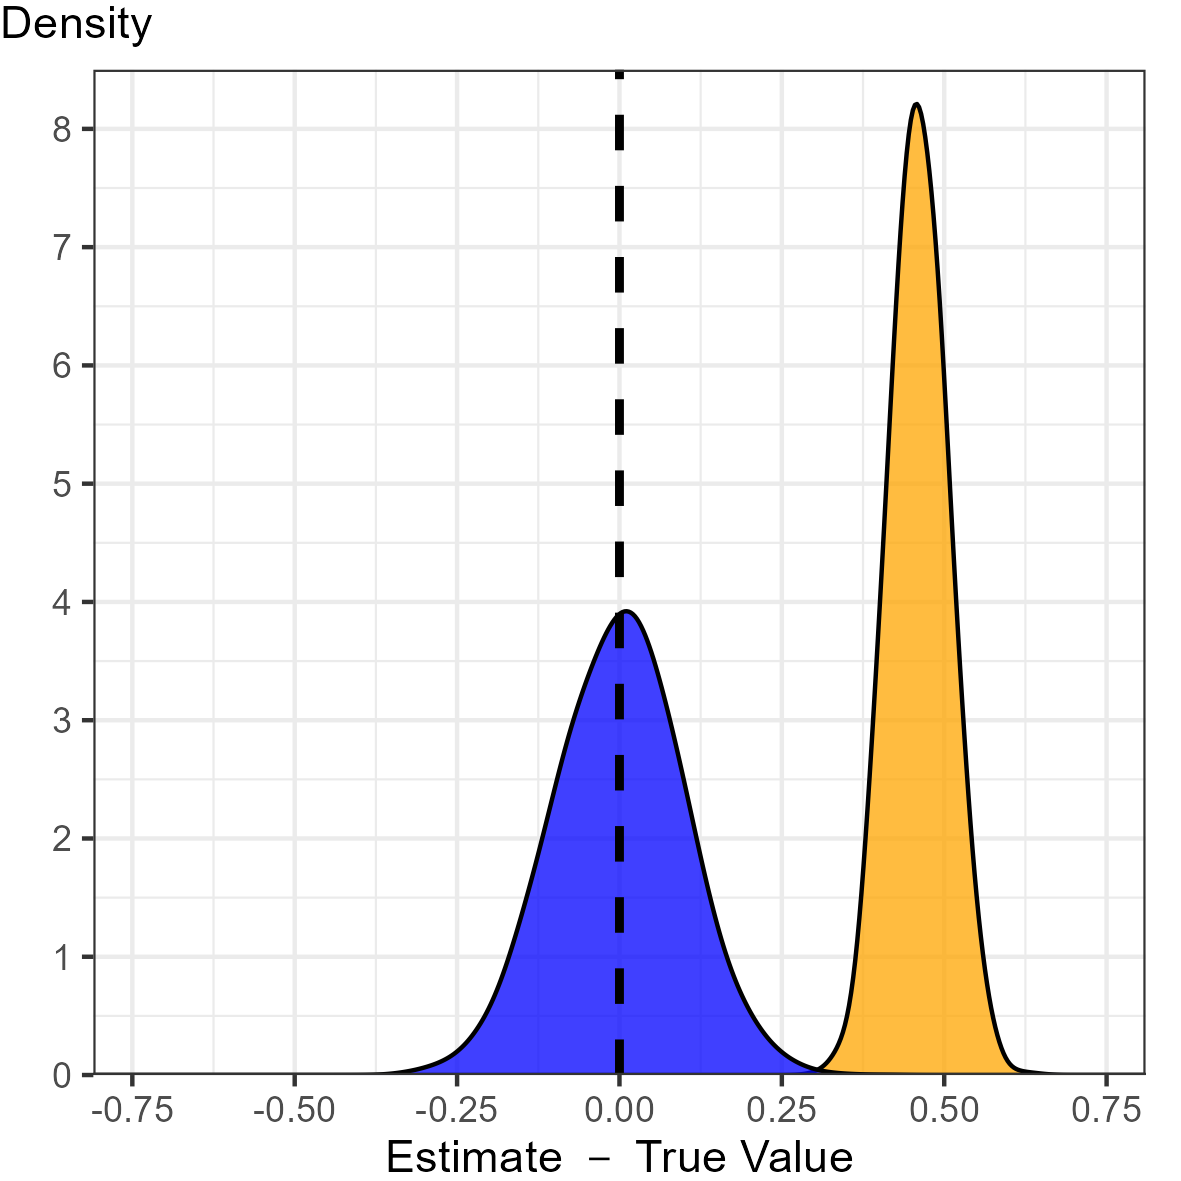
\includegraphics[width=\textwidth]{
                    ../text/sections/figures/normal-indirect-dist.png}
            \end{subfigure}
        \end{figure}
    }}
\end{frame}
%-------------------------------------------------------------------------------
%\section{4. Oregon}
%%-------------------------------------------------------------------------------
%\begin{frame}
%    \frametitle{4. Returning to Oregon}
%    Conventional CM estimates lottery effects as mostly direct, $\approx 0$ healthcare.
%    \vskip0.5cm
%    
%    \begin{figure}
%        %\caption{CM Estimates in the Oregon Health Insurance Experiment.}
%        %\vskip-0.25cm
%        \centering
%        \includegraphics[width=0.9\textwidth]{
%            ../text/sections/figures/mediation-health-placeholder.png}
%    \end{figure}
%\end{frame}
%%-------------------------------------------------------------------------------
%\begin{frame}
%    \frametitle{4. Returning to Oregon}
%    Using my MTE model, with regular healthcare location as an excluded IV, restores indirect effect through increased \textcolor{ForestGreen}{healthcare visitation}.
%    \vskip0.5cm
%    
%    \begin{figure}
%        %\caption{CM Estimates in the Oregon Health Insurance Experiment.}
%        %\vskip-0.25cm
%        \centering
%        \includegraphics[width=0.9\textwidth]{
%            ../text/sections/figures/mediation-health.png}
%    \end{figure}
%\end{frame}
%%-------------------------------------------------------------------------------
\begin{frame}
    \frametitle{Conclusion}
    \begin{enumerate}
        \item Conventional CM has selection bias in observational (economic) settings
        \item MTE-based model avoids selection bias
        \item Meaningful indirect (healthcare) and direct (psychological) effects in Oregon Health Insurance Experiment, with wide confidence intervals showing true uncertainty in mechanism explanations.
    \end{enumerate}
    \vfill
    \textbf{Questions?}
\end{frame}
%-------------------------------------------------------------------------------
\end{document}
